\section{Auswertung}
\subsection{Bestimmung der g-Faktoren und Horizontalkomponente der Erdmagnetfeld}
Zu Beginn werden die lokale horizontal Komponente des Erdmagnetfeldes und die Lande-Faktoren $g_F$ der Rb-Isotope, welche in der Dampfzelle enthalten sind, ermittelt.
Dafür werden die an der HF-Spule angelegten Frequenzen $\nu$ gegen die magnetischen Feldstärken $B$ in der jeweiligen Resonanz aufgetragen. Mittels einer linearen Ausgleichsrechnung werden die $g_F$ aus der Steigung errechnet und die horizontal Komponente des Erdmagnetfeldes als Ordinate identifiziert.

Um die gemessenen Stromstärken in ein Magnetfeld umzurechnen, wurde der bekannte Zusammenhang für Helmholzspulen

\begin{equation}
B = \mu_0 \frac{8NI}{\sqrt{125} r}
\end{equation}

genutzt.

\begin{figure}[h]
\centering
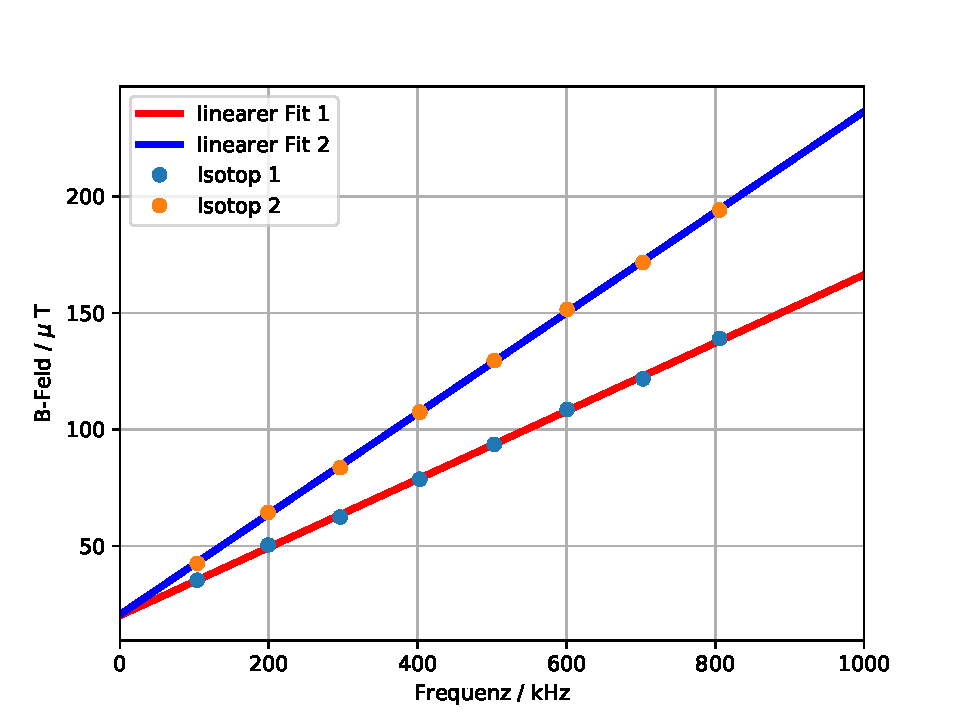
\includegraphics[scale=0.8]{img/plotLande.pdf}
\caption{Ausgleichsrechnung zur Bestimmung der Lande Faktoren der Rb-Isotope und der lokalen horizontal Komponente des Erdmagnetfeldes}
\label{abb:gfak}
\end{figure}

Mit dem Ansatz

\begin{equation}
B(\nu) = A\nu + B_\text{Erd}
\end{equation}

folgt aus der Ausgleichsrechnung gemäß \autoref{abb:gfak} folgende Werte für die Koeffizienten $A$ und $B_\text{Erd}$:

\begin{table}\centering\begin{tabular}{ccc} \toprule 
\centering
\caption{Ergebnisse für die Koeffizienten A und B der Ausgleichsrechnung.}
\label{tab:isoFit}
 & A / $\mu$T/kHz  & B / $\mu$T \\ \midrule
Isotop 1 & 0.146 $\pm$ 0.001 & 20.1 $\pm$ 0.7 \\
Isotop 2 & 0.216 $\pm$ 0.001 & 20.5 $\pm$ 0.6 \\
\bottomrule
\end{tabular}
\end{table}

Durch Koeffizientenvergleich mit Gleichung \ref{eq:ausgleich} folgt für die Lande Faktoren

\begin{equation} 
g_{F1} = 0.488\pm0.005\,
label{eq:resG1}
\end{equation} 


und

\begin{equation} 
g_{F2} = 0.331\pm0.002\,
label{eq:resG2}
\end{equation} 


Außerdem lässt sich aus der Ordinate die Horizontalkomponente des Erdmagnetfeldes bestimmen,
welche sich zu

\begin{equation} 
B_\text{h} = 20.3\pm0.5\,\mu\text{T}
\end{equation} 


errechnet. Für das abschließende Ergebnis der Horizontaltkomponente des Erdmagnetfeldes, wurde der Mittelwert über beide Einzelergebnisse der Ausgleichsrechnung berechnet.

\subsection{Bestimmung der Kernspins}
Für die Kernspins der Rb-Isotope gelten folgende Zusammenhänge: $S = J = \frac{1}{2} , L = 0$ sowie $F = I - J$ und $g_e = 2.0023$ \cite{landeE-}. Ferner wird
der Zusammenhang dieser Größen durch \ref{eq:g} bestimmt. Werden o.g. Annahmen berücksichtigt vereinfacht sich \ref{eq:g} zu

\begin{equation}
I = \frac{g_e}{2g_F} - \frac{1}{2}.
\end{equation}

Unter Verwendung von \ref{eq:resG1} und \ref{eq:resG2} berechnen sich die Kernspins der Isotope zu

\begin{equation}
I_{Isotop1} = 1.55 \pm 0.02 
\label{eq:result1}
\end{equation}

und

\begin{equation}
I_{Isotop2} = 2.53 \pm 0.02
\label{eq:result2}
\end{equation}

Die errechneten Kernspins werden mit den Kernspins der Rubidiumisotope von \cite{coreSpin} verglichen. Dieser Vergleich lässt den Schluss zu,
dass es sich bei \ref{eq:result1} um $Rb_{87}$ und bei \ref{eq:result2} um $Rb_{85}$ handelt.

\subsection{Bestimmung des Isotopenverhältnisses}
In Abbildung \ref{resonanz} ist das Signalbild dargestellt, welches die Resonanzen zu festen
HF-Frequenzen und variablen B-Feld zeigt.

\begin{figure}[h]
\centering
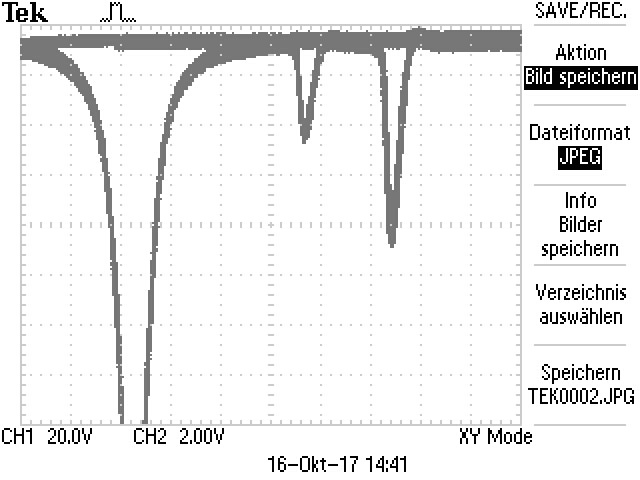
\includegraphics[scale=0.8]{img/TEK0002.JPG}
\caption{Abbildung der Resonanzen}
\label{resonanz}
\end{figure}


Aus dem Amplitudenverhältnis der Resonanzen wird das Isotopenverhältnis in der
Dampfzelle ermittelt. Dafür wird die Tiefe h der Resonanzen in Pixel bestimmt.
Eine Messung der Tiefe der Resonanzen mit gimp liefert für die erste Resonanz (von links)

\begin{equation} 
h_1 = 108.0\pm1.1\,\text{px}
\end{equation} 


für die zweite Resonanz

\begin{equation} 
h_2 = 213.0\pm2.1\,\text{px}
\end{equation} 


und für das Amplitudenverhältnis

\begin{equation} 
r = 0.507\pm0.007\,
\end{equation} 


Bei der Kalkulation des Amplitudenverhältnisses wurde ein Ablesefehler von 1 Prozentpunkt
angesetzt.

\subsection{Abschätzung des quadratischen Zeemann-Effektes}
Für starke Magnetfelder verhält sich die Übergangsenergie $U_{HF}$ nicht mehr proportional zu B. Um diese Abweichung zu berücksichtigen, ist es notwendig Terme höherer Ordnung zu betrachten.
Für das Magnetfeld wird eine Feldstärke von $B = 200 \mu T$ angesetzt. Außerdem wird $g_{F,85} = 0,488$, $g_{F,87} = 0,331$, $M_F = 0$, 
$EHyp_{85} = 2,01 \cdot 10^{-24}$ und $EHyp_{87} = 4,53 \cdot 10^{-24}$ \cite{FP} verwendet. Mit Hilfe dieser Werte wird \ref{eq:qze} ausgewertet. Für $Rb_{85}$ folgt

\begin{equation}
U_{HF,85} = 9,05 \cdot 10^{-28} + 4,08 \cdot 10^{-31}
\end{equation}

und für $Rb_{87}$ folgt

\begin{equation}
U_{HF,87} = 6,14 \cdot 10^{-28} + 8,32 \cdot 10^{-32}
\end{equation}
.

\subsection{transiente Effekte}
Im folgenden werden die transienten Effekte betrachtet. Ein typisches Signalbild ist Abbildung \ref{sigPic} zu entnehmen.

\begin{figure}[h]
\centering
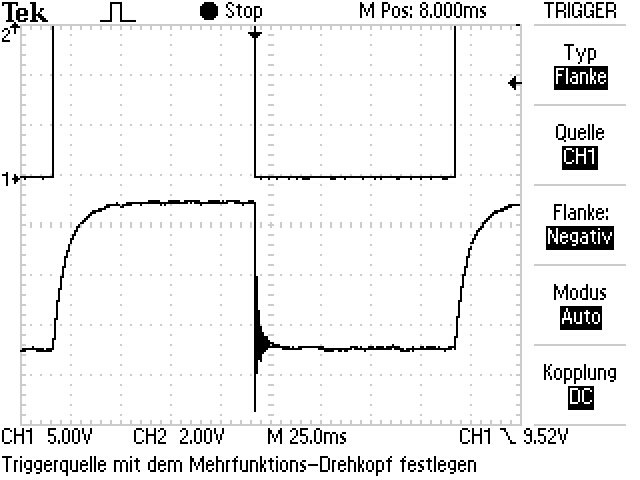
\includegraphics[scale=0.8]{img/TEK0019.JPG}
\caption{Signalbild}
\label{sigPic}
\end{figure}

Es wird die Periode gegen die RF-Amplitude aufgetragen und anschließend eine Ausgleichsrechnung mit Hilfe der Funktion

\begin{equation}
f(x) = A + \frac{B}{(x+C)^{-1}}
\end{equation}

durchgeführt.

Es ergeben sich die Abbildungen \ref{trans1} und \ref{trans2} mit den dazugehörigen Fitparametern in Tabelle 2 und Tabelle 3.

\begin{figure}[h]
\centering
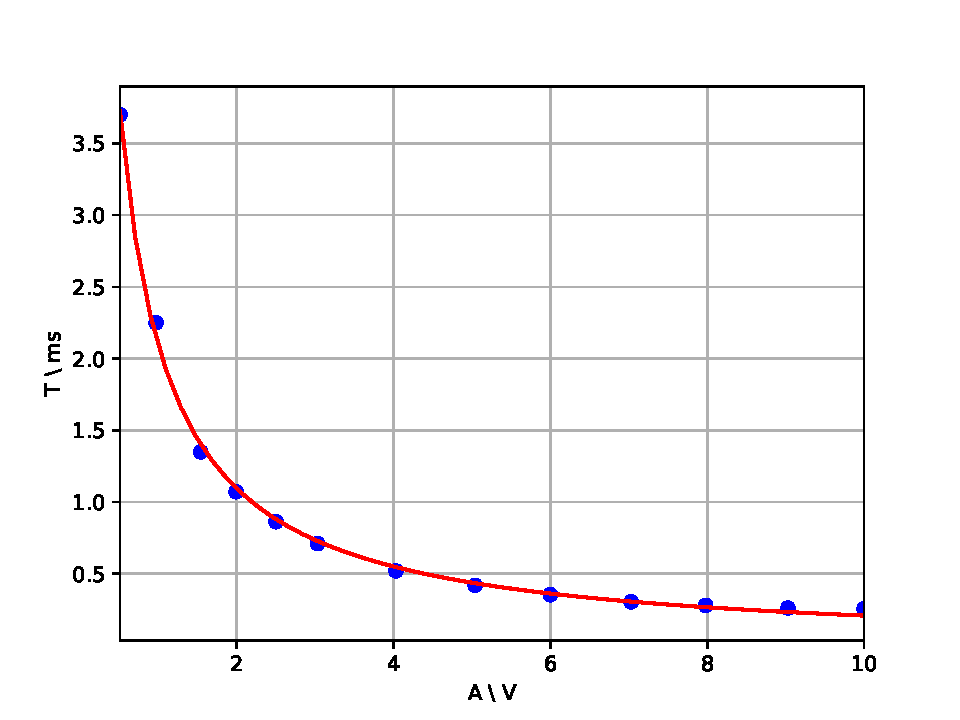
\includegraphics[scale=0.8]{img/trans1.pdf}
\caption{Ausgleichsrechnung zum transienten Verhalten von $Rb_{85}$}
\label{trans1}
\end{figure}

\begin{figure}[h]
\centering
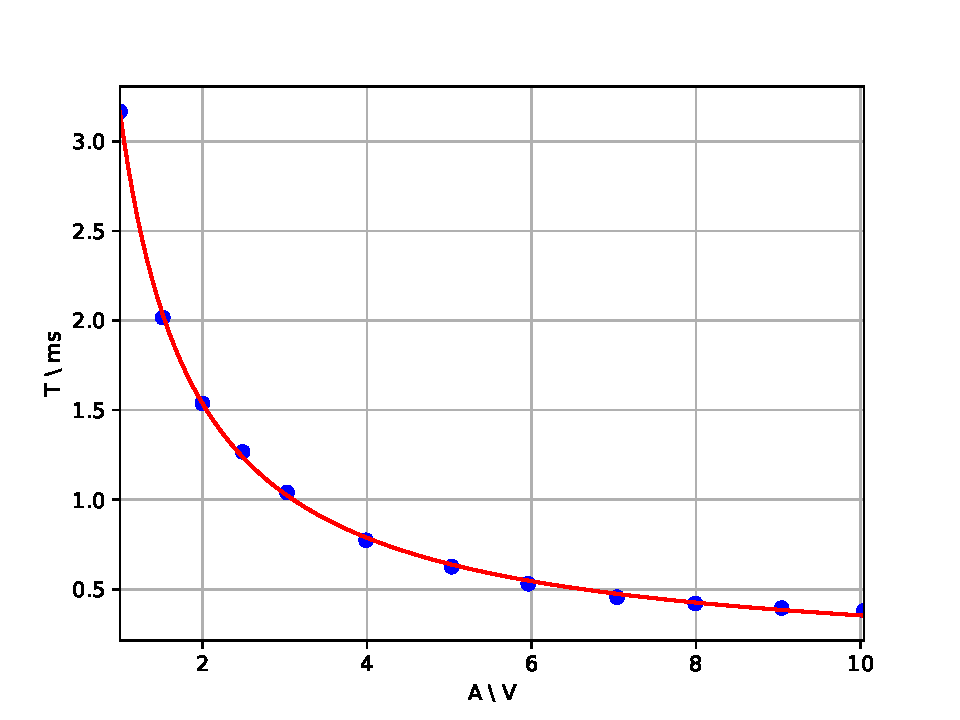
\includegraphics[scale=0.8]{img/trans2.pdf}
\caption{Ausgleichsrechnung zum transienten Verhalten von $Rb_{87}$}
\label{trans2}
\end{figure}

\begin{table}[h!]
\centering
\begin{tabular}{cc} \toprule
\centering
A & -0,03 $\pm$ 0,03 \\
B & 2,4 $\pm$ 0,1 \\
C & -0,13 $\pm$ 0,03 \\
\bottomrule
\end{tabular}
\label{x}
\caption{Ausgleichsrechnung für $Rb_{85}$}
\end{table}

\begin{table}[h!]
\centering
\begin{tabular}{cc} \toprule
\centering
A & 0,07 $\pm$ 0,01 \\
B & 2,79 $\pm$ 0,07 \\
C & 0,09 $\pm$ 0,02 \\
\bottomrule
\end{tabular}
\label{y}
\caption{Ausgleichsrechnung für $Rb_{87}$}
\end{table}

Der Quotient der Fitparameter B der beiden Ausgleichsrechnungen liefert

\begin{equation}
\frac{b_{87}}{b_{85}} = 1,17 \pm 0,06
\end{equation}
.
